\section{Epilepsy data}


\begin{figure}[!htbp]
\minipage{0.5\textwidth}%
\centering
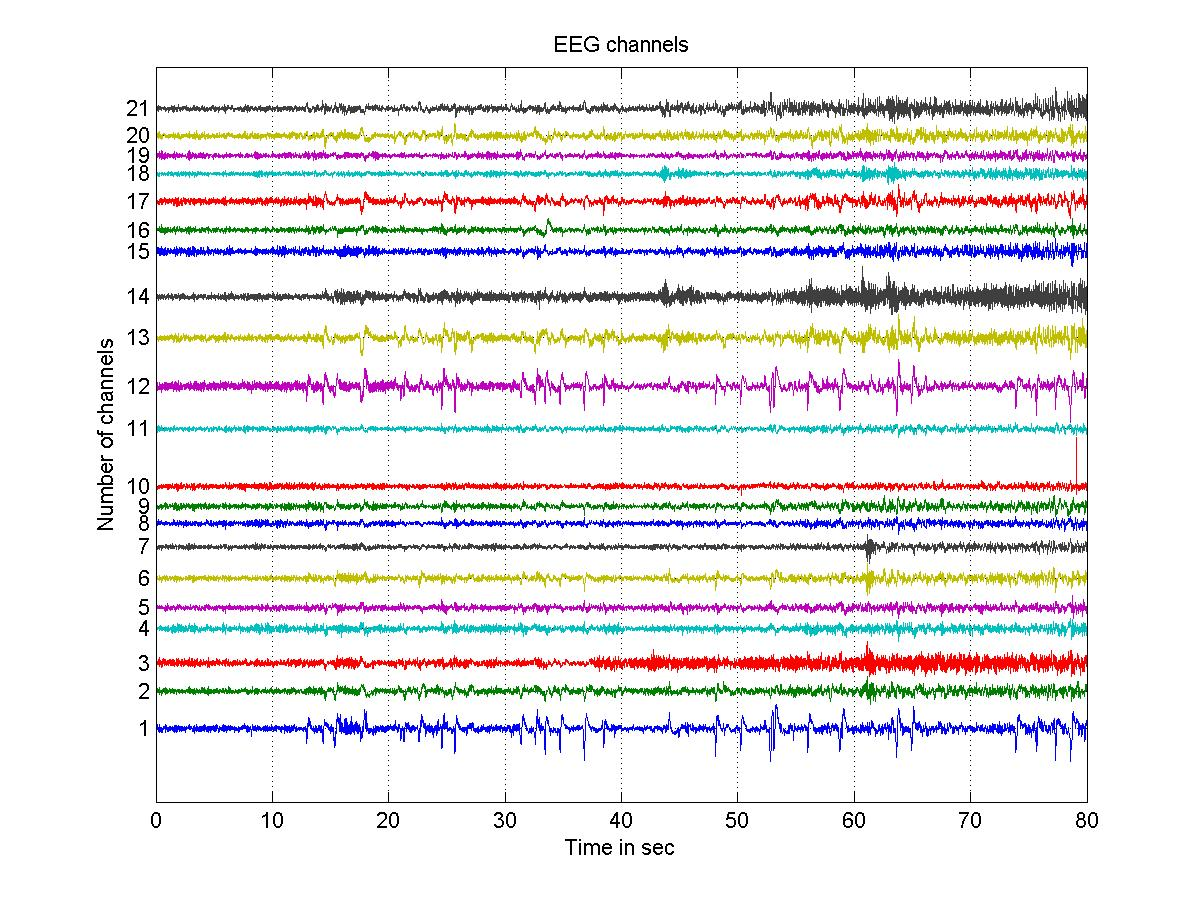
\includegraphics[width=1\linewidth]{300.jpg}
\subcaption{EEG signal}
\endminipage\hfill
\minipage{0.5\textwidth}%
\centering
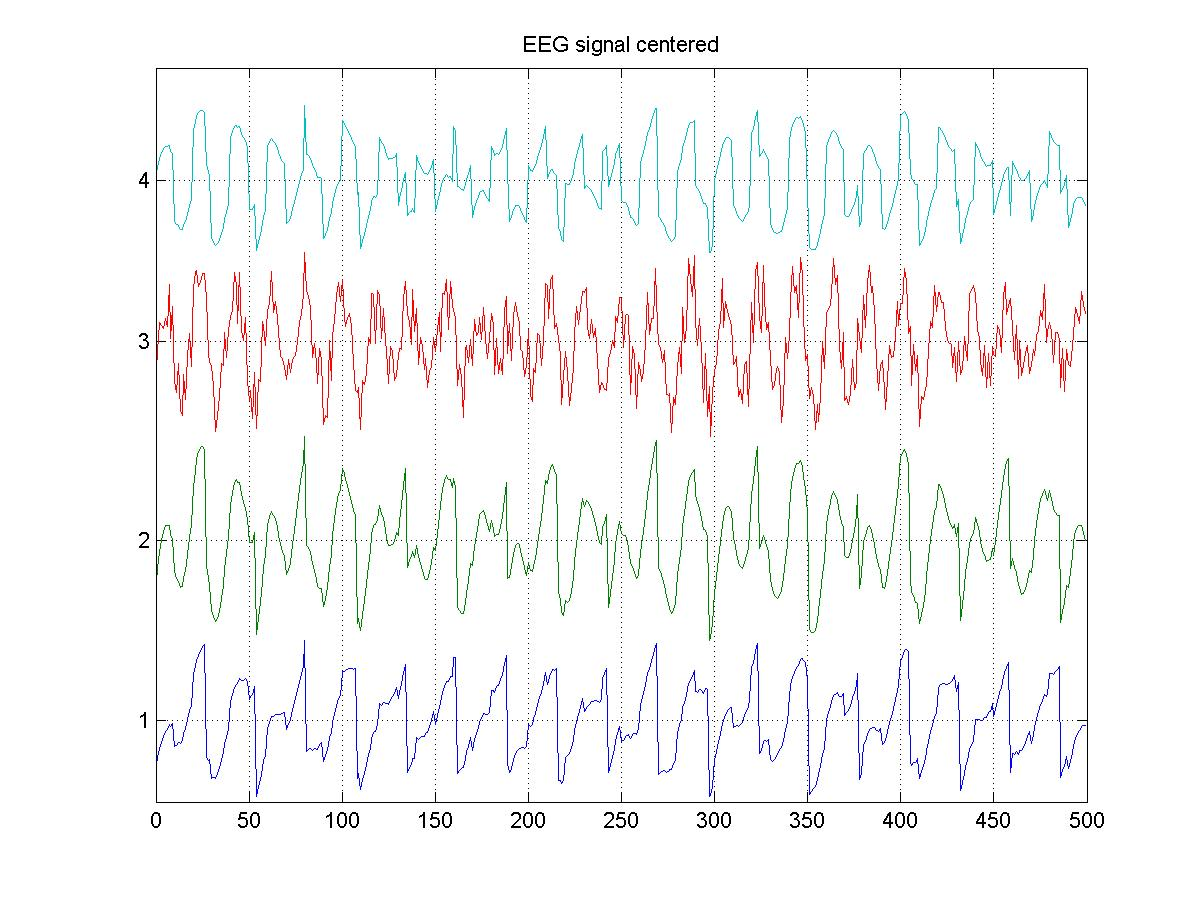
\includegraphics[width=1\linewidth]{301.jpg}
\subcaption{Unfolded Tensor.}
\endminipage\hfill
\caption{EEG signal and its tensor of 21*24*500 dimensions unfolded into  504x500 matrix}
\end{figure}

The EEG data set is structured into different channel data over a time course of 80 sec. An epileptic seizure has been detected at around t=52 sec. In order to map this signal into a head model, BSS has to be performed over the dataset. Hereby the normal brain activity has to be separated from the epilepsy. Tensorisation has to be formed via wavelet transform. The outcome will be a third order tensor where its respective orders are time, frequency and the number of channels. 

In order to estimate the rank of this tensor, the performance of CPD has been tested over different rank trials. In figure \ref{CPD-4} the plots clearly testify the fastest convergence for a rank two computation. 

\begin{figure}[!htbp]
\centering
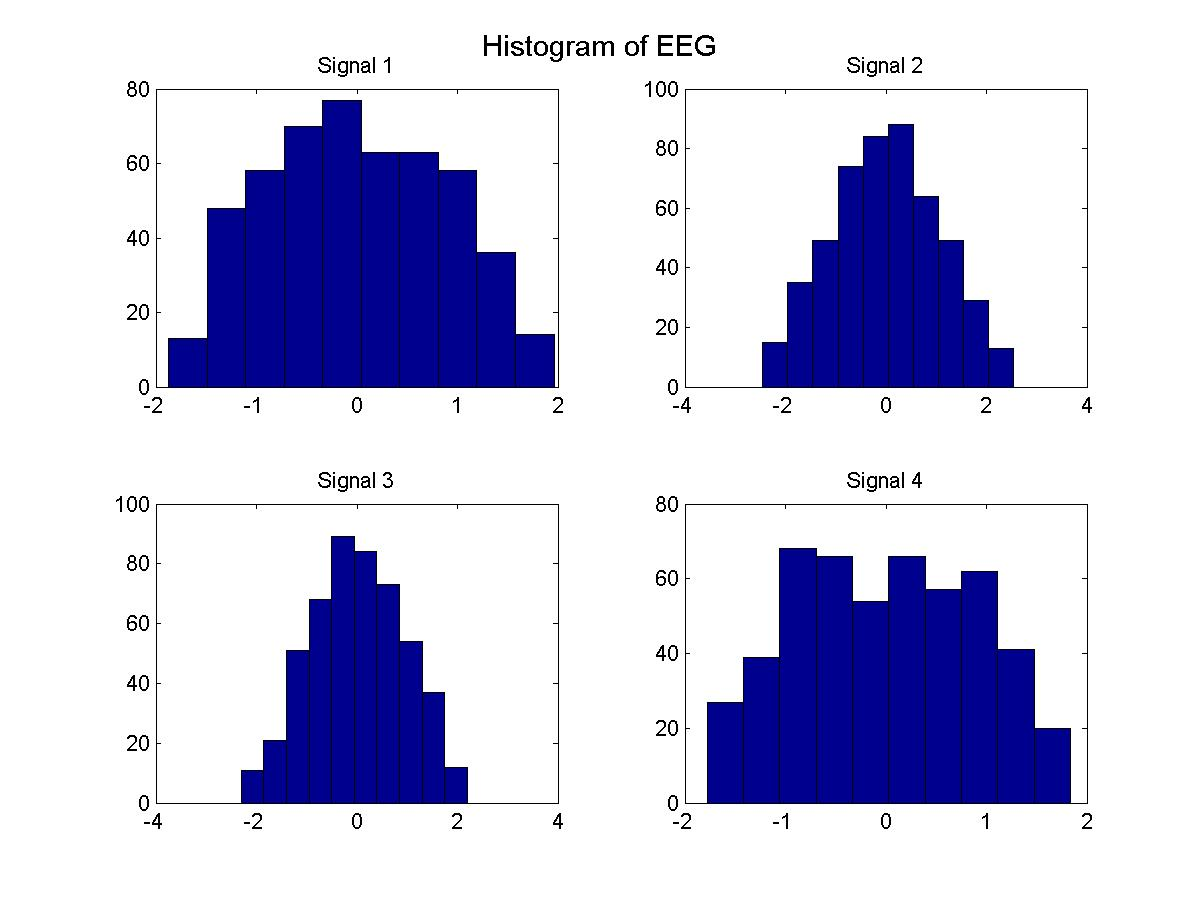
\includegraphics[width=0.5\linewidth]{304.jpg}
\caption{CPD performance}\label{CPD-4}
\end{figure}


Therefore the number of rank one tensor correspond to distinct uncorrelated event encoded into the EEG signals. Epilepsy as the first component together with the normal brain activity signals are both superimposed. Since CPD ensures a unique BSS the event are efficiently separated and their potential distribution into a spherical head model produces completely different potential map. 

Epilepsy is mostly associated with high frequency variations in the EEG signals whereas a brain activity stands mostly a low frequencies. 

In order to testify this the first mode of the decomposition has been plotted in figure \ref{AC1} and \ref{AC2}. The frequency component in figure \ref{AC1} for the highest variation in frequency is quite irregular and chaotic behaviour. This has been associated to epilepsy. This is also the case in higher order component of the temporal signature in figure \ref{AC2} where a more pronounced chaotic behaviour is outlined for the seizure.



\begin{figure}[!htbp]
\minipage{0.5\textwidth}%
\centering
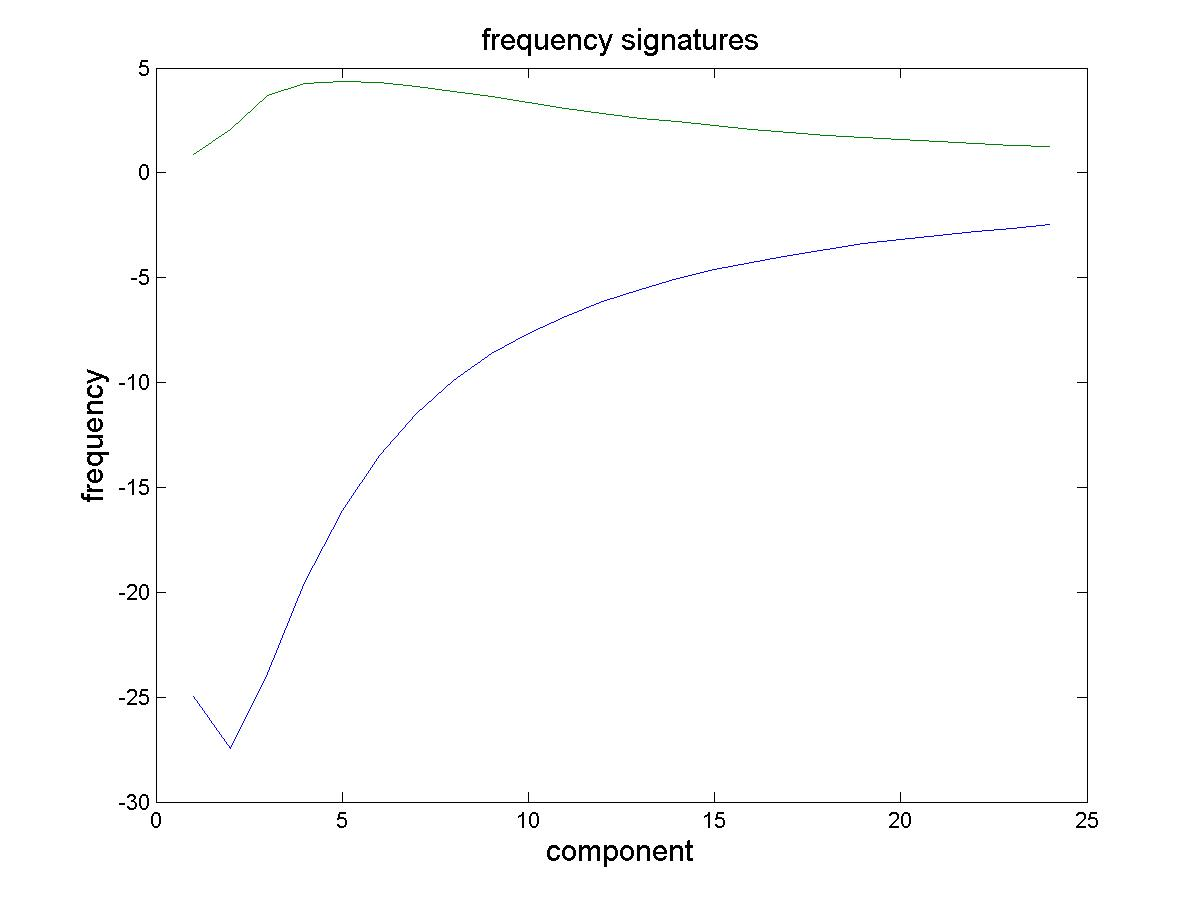
\includegraphics[width=1\linewidth]{302.jpg}
\subcaption{Frequency components}\label{AC1}
\endminipage\hfill
\minipage{0.5\textwidth}%
\centering
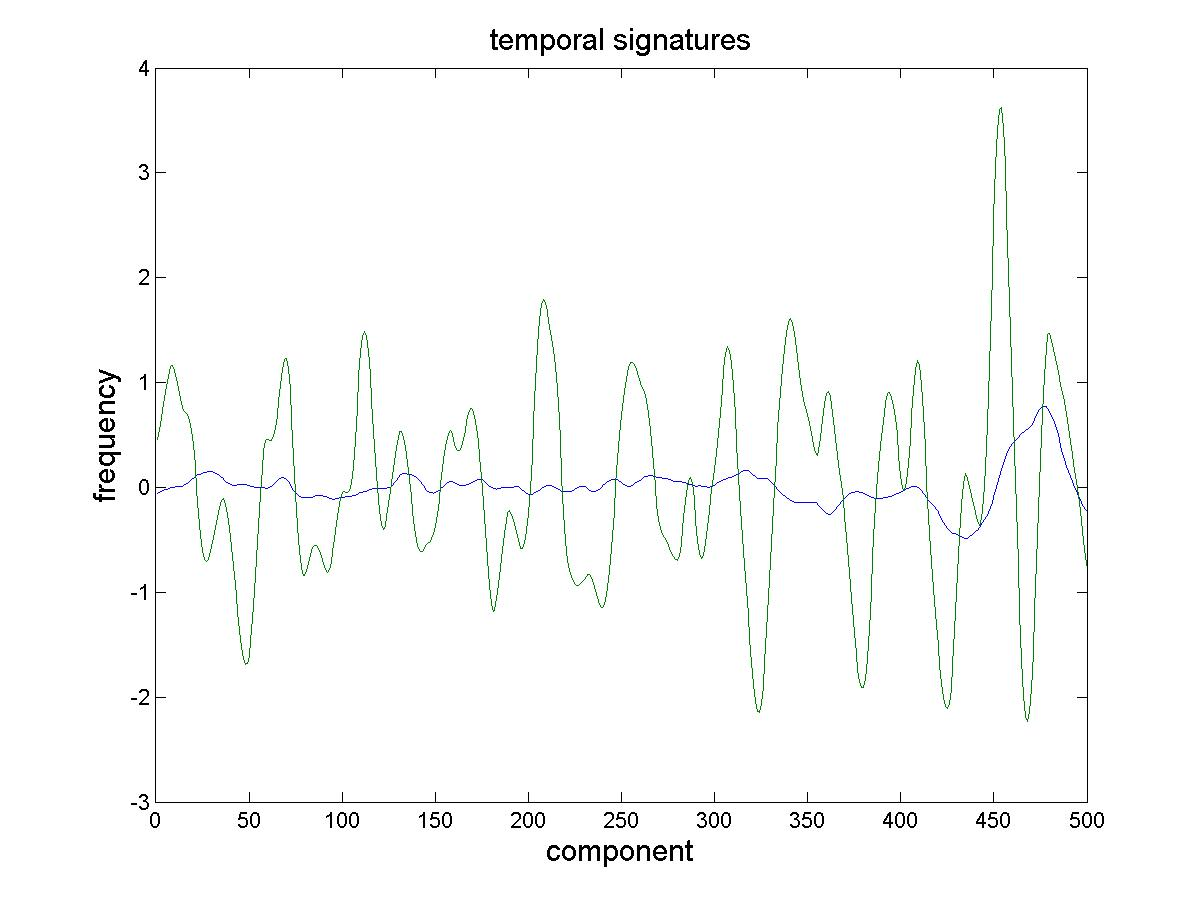
\includegraphics[width=1\linewidth]{303.jpg}
\subcaption{Time course activity}\label{AC2}
\endminipage\hfill
\caption{Plots of distinct events}
\end{figure}

These two event are mapped into a spherical head model in figure \ref{AC3} is the seizure located on top of the head whereas the second component which is the normal brain activity is potential distribution in figure \ref{AC4}.


\begin{figure}[!htbp]
\minipage{0.5\textwidth}%
\centering
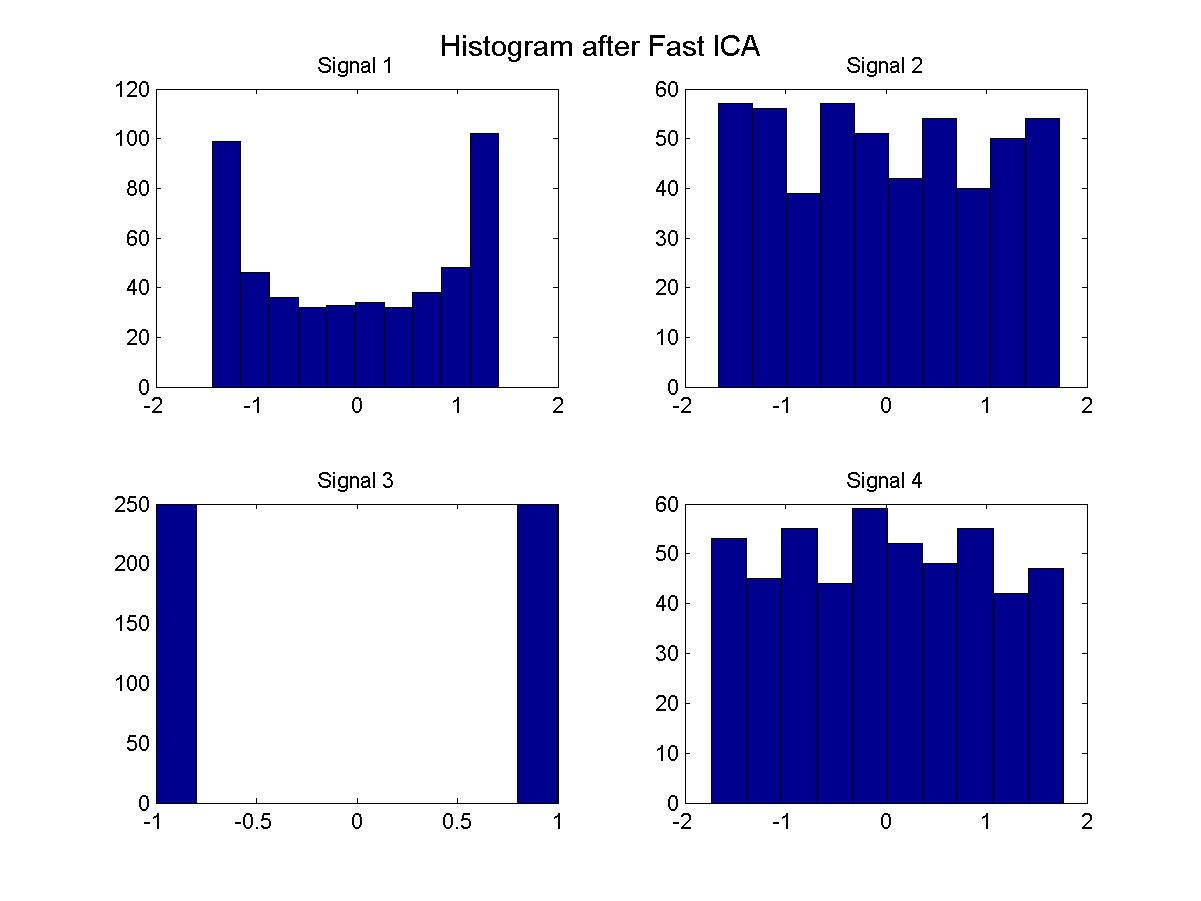
\includegraphics[width=1\linewidth]{305.jpg}
\subcaption{Seizure.}\label{AC3}
\endminipage\hfill
\minipage{0.5\textwidth}%
\centering
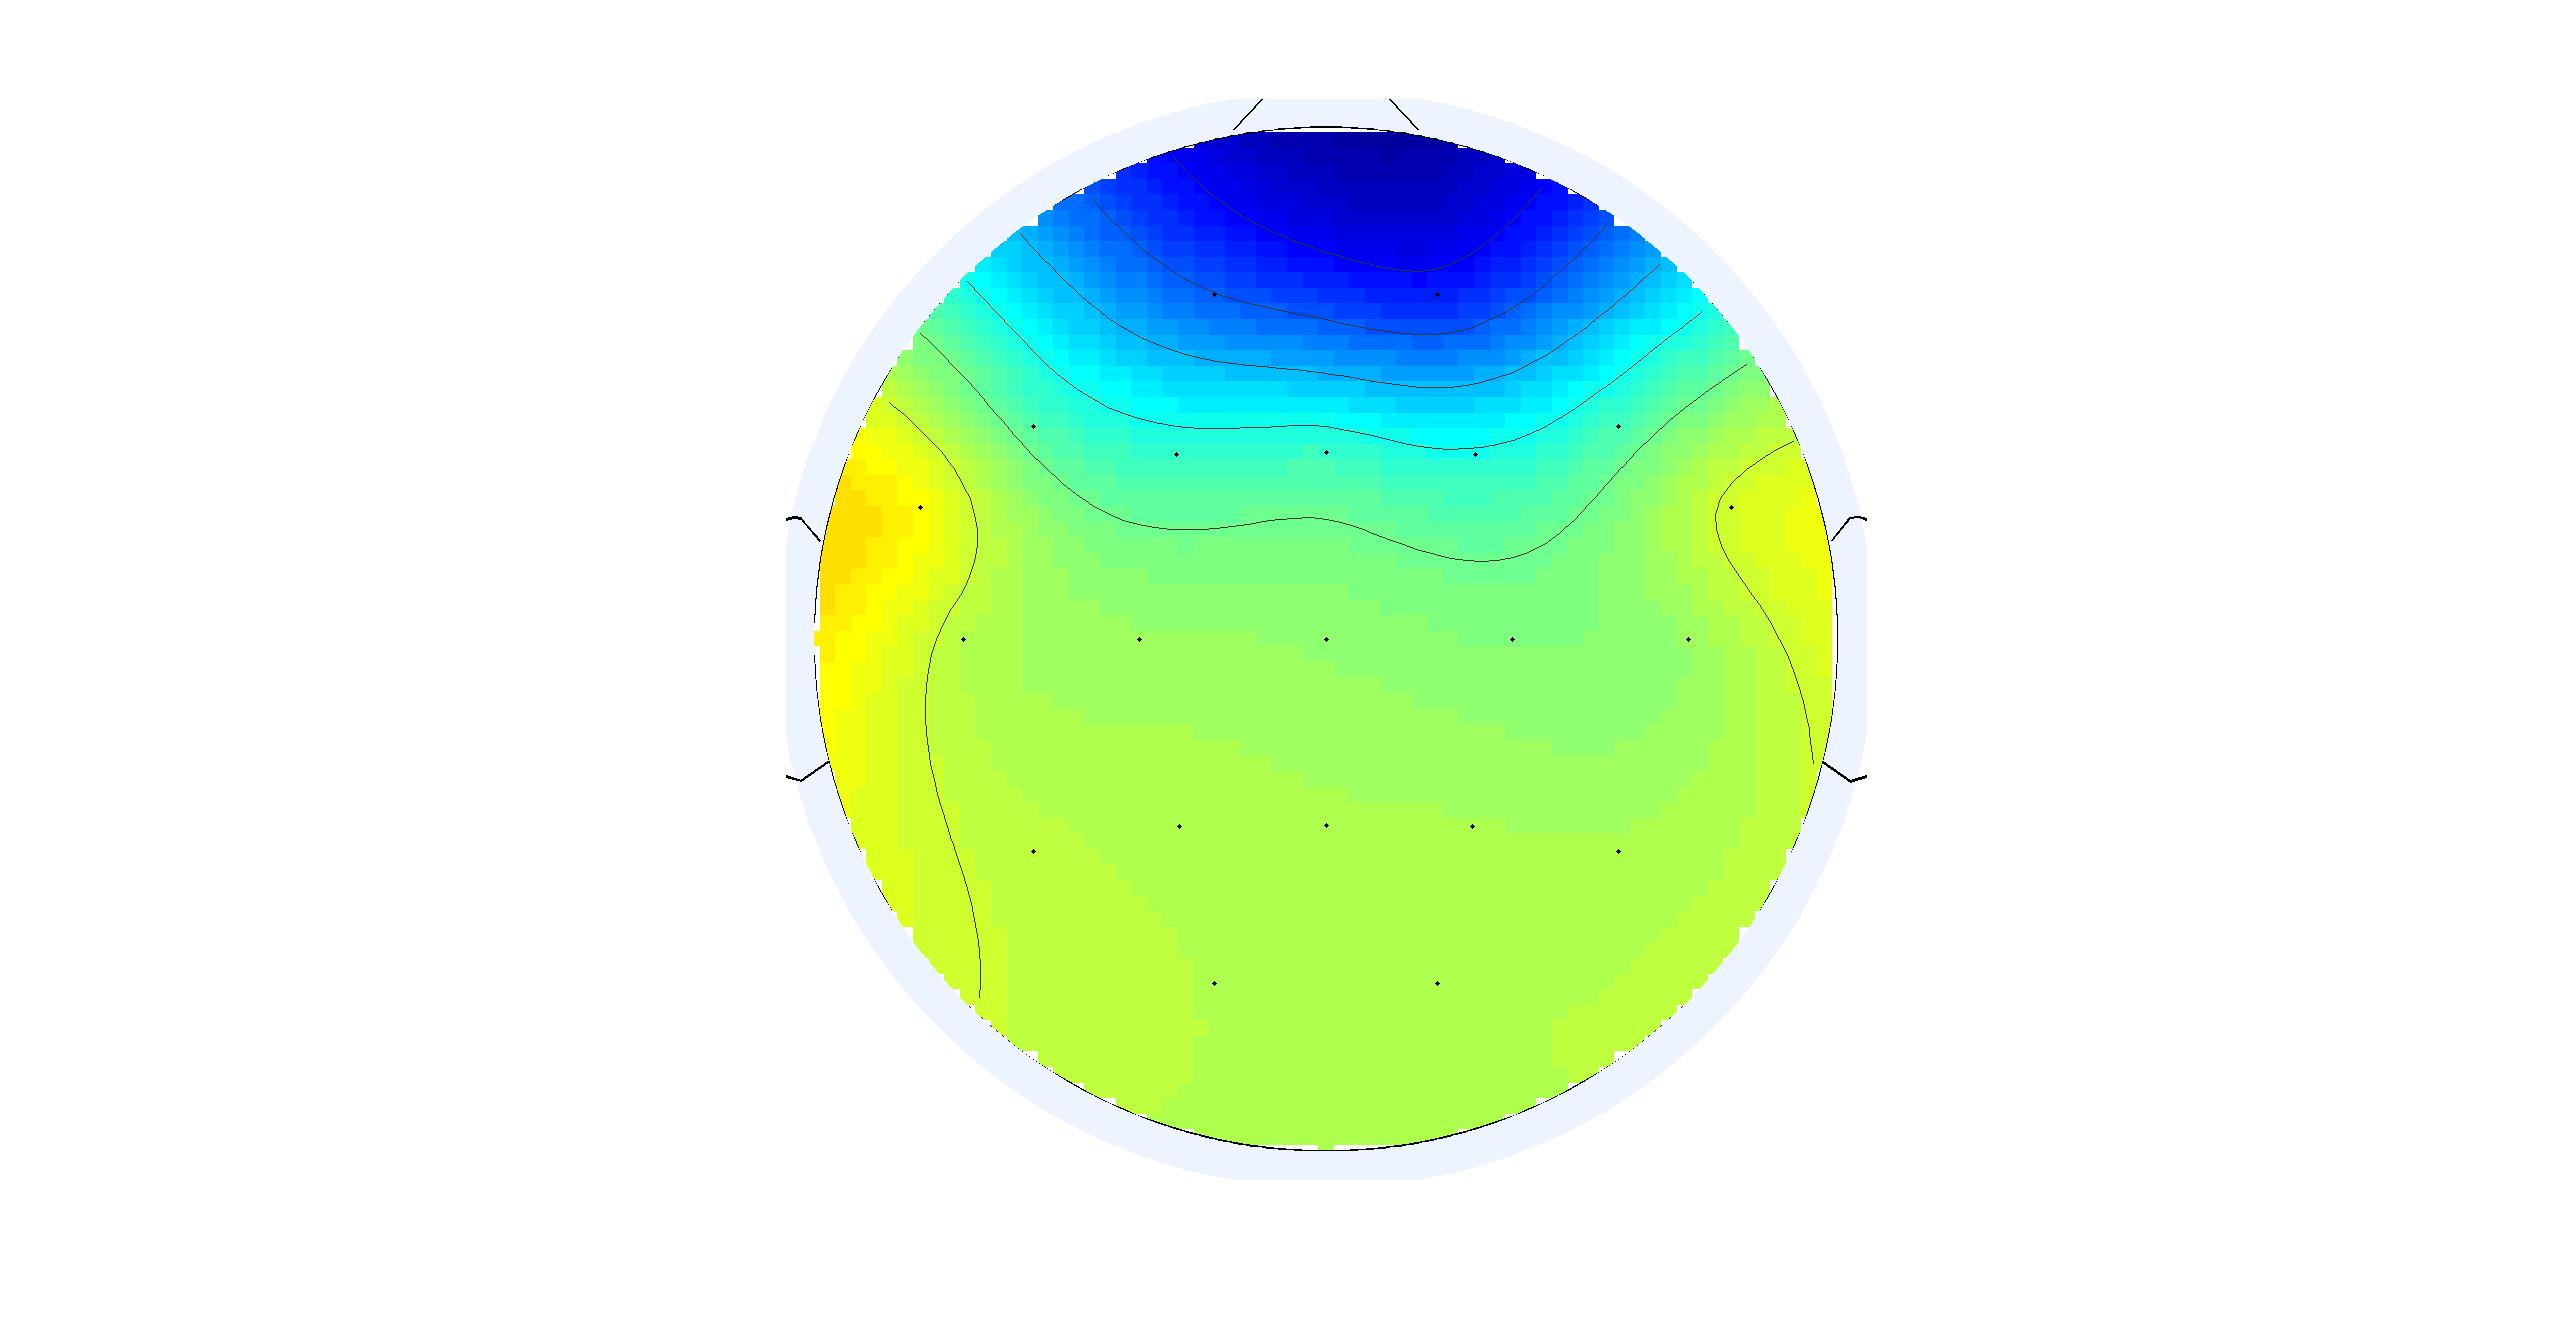
\includegraphics[width=1\linewidth]{307.jpg}
\subcaption{Normal activity}\label{AC4}
\endminipage\hfill
\caption{Potential distribution of these two events}
\end{figure}
